\documentclass{article} % For LaTeX2e
\usepackage{naaclhlt2016}
\usepackage{times}
\usepackage{latexsym}
\usepackage{hyperref}
\usepackage{url}
\usepackage{amsmath,amsthm,amsfonts}
\usepackage{multirow,multicol}
\usepackage{xspace}
\usepackage{tikz}
\usepackage{natbib}
\usetikzlibrary{shapes,backgrounds,patterns}


\newcommand{\Prob}{\mathbb{P}}
\newcommand{\todo}[1]{{\bf [[}\textcolor{blue}{ todo: #1}{\bf ]]}}
\newcommand{\fix}{\marginpar{FIX}}
\newcommand{\new}{\marginpar{NEW}}

% named as such because `\arg1' apparently isn't valid
\newcommand{\argOne}{\emph{arg1}\xspace}
\newcommand{\argTwo}{\emph{arg2}\xspace}


% \title{Broad Coverage Knowledge Base Construction using Cross-Lingual Transfer}
%\title{No KB? No Problem! Transfer Learning for Multilingual Relation Extraction}
\title{Multilingual Relation Extraction using \\Compositional Universal Schema}
%\title{Transfer Learning for Multilingual \\Knowledge Base Construction}
% \title{Broad Coverage Knowledge Base Construction using Multilingual Embeddings}

\author{Patrick Verga, David Belanger, Emma Strubell, Benjamin Roth \& Andrew McCallum \\
College of Information and Computer Sciences\\
University of Massachusetts, Amherst\\
% Amherst, MA 01002, USA \\
\texttt{\{pat, belanger, strubell, beroth, mccallum\}@cs.umass.edu} \\
}


%\iclrfinalcopy % Uncomment for camera-ready version

\begin{document}


\maketitle

\begin{abstract}
When building a knowledge base (KB) of entities and relations from multiple structured KBs and text, \emph{universal schema} represents the union of all input schema, by jointly embedding all relation types from input KBs as well as textual patterns expressing relations.  In previous work, textual patterns are parametrized as a single embedding, preventing generalization to unseen textual patterns.  In this paper we employ an LSTM to compositionally capture the semantics of relational text.  We dramatically demonstrate the flexibility of our approach by evaluating in a multilingual setting, in which the English training data entities overlap with the seed KB, but the Spanish text does not.  Additional improvements are obtained by tying word embeddings across languages.  In extensive experiments on the English and Spanish TAC KBP benchmark, our techniques provide substantial accuracy improvements.  Furthermore we find that training with the additional non-overlapping Spanish also improves English relation extraction accuracy.  Our approach is thus suited to broad-coverage automated knowledge base construction in low-resource languages and domains.
\end{abstract}


% intro + background

\section{Introduction\label{introduction}}


\subsection {Universal Schema}
The goal of automatic knowledge base construction (AKBC) is to build a structured knowledge base (KB) of facts using a noisy corpus of raw text evidence, and perhaps an initial seed KB to be augmented~\citep{NELL,yago,freebase}. AKBC supports downstream reasoning at a high level about extracted entities and their relations, and thus has broad-reaching applications to a variety of domains.
An effective approach to AKBC is Universal Schema.
Universal Schema embeds textual patters and knowledge bases into a shared space in order to reason over relations and entity pairs.
A low dimensional embedding is learned for each entity pair and each relation type using matrix factorization.
The model is then able to infer relations between entities as the dot product between the two entity pair and relation type vectors.

Unfortunately, this formulation limits the generalization of the model.
In its original form, Universal Schema can only reason about entity pairs and textual relations explicitly seen at training time.

\subsection {Compositional Universal Schema}

Recently Universal Schema has been extended to deal with compositional representations of textual relations \citep{toutanova2015representing,verga2015multilingual}
Compositional Universal Schema has two main advantages over explicit modeling of textual patterns.
The first is tt allows for the model to share statistics between very similar patterns.
Instead of modeling the text pattern 'lives in the city' and 'lives in the city of' as distinct atomic units, they can instead be composed compositionally of the same word embeddings.
Second, and even more importantly, Compositional Universal Schema allows us to generalize to all possible textual patterns, allowing us to reason over any arbitrary text.

\begin{figure}[h]
\caption{Top : Universal Schema expresses each textual pattern as an atomic unit \protect\citet{riedel2010modeling}.
Bottom : Compositional Universal Schema uses an lstm to encode each textual relation \protect\cite{verga2015multilingual}. }
\centering
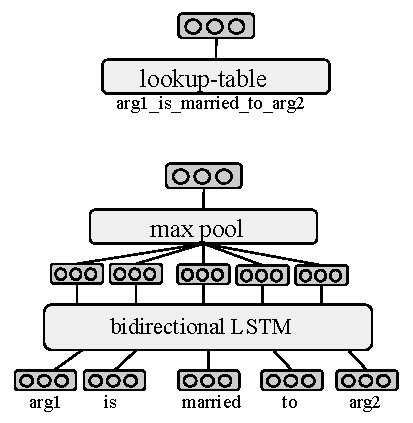
\includegraphics[scale=.68]{relation-models}
\end{figure}

\subsection {Universal Schema without Entity Embeddings}

While Compositional Universal Schema addresses reasoning over arbitrary textual patterns, it is still limited to reasoning over entity pairs seen at training time.
\citet{verga2015multilingual} approach this problem by using Universal Schema as a sentence classifier - directly comparing a textual relation to a kb relation to perform relation extraction.
However, this approach is unsatisfactory for two reasons.
The first is that this creates an inconsistency between training and testing, as the model is trained to predict compatibality between entity pairs and relations and not relations directly.
Secondly, it considers only a single piece of evidence while making its prediction.

The learned entity pair can be seen as a sumamrization of all relations for which that entity pair was seen.


Rather than modeling each entity pair as an explicit vector, we instead treat each entity pair as an aggregate function over each of its relation types.
This allows us to trivially extend to unseen entity pairs, have a direct link to provenance, and allocate a variable number of parameters per entity pair.


\subsection {Entities vs Entity Pairs}

A knowledge base is naturally described as a graph, in which entities are nodes and relations are labeled edges~\citep{yago,freebase}.
In the case of \emph{knowledge graph completion}, the task is akin to link prediction, assuming an initial set of (\emph{s, r, o}) triples.
See~\citet{nickel2015review} for a review.
No accompanying text data is necessary, since links can be predicted using properties of the graph, such as transitivity.
In order to generalize well, prediction is often posed as low-rank matrix or tensor factorization.
A variety of model variants have been suggested, where the probability of a given edge existing depends on a multi-linear form~\citep{rescal,DBLP:journals/corr/Garcia-DuranBUG15,bishan,transe,wang2014knowledge,lin2015learning}, or non-linear interactions between $s$, $r$, and $o$~\citep{socherkb}.

These models all operate at the level of entities rather than entity pairs.
Entity-based models have recall advantages over entity pairs.
For any two entities, the model is able to make predictions even if there is no information regarding the explicit entity pair.
However, this essentially reduces to type clustering as every action star would have a high probability for every action movie.

Entity pairs on the other hand have higher precision.
Both~\citet{toutanova2015representing} and~\citet{limin} observed that the entity pair model outperforms entity models in cases where the entity pair was seen at training time.
This is particularly important when jointly embedding text and knowledge bases.
By leveraging large amounts of unlabeled text, Universal Schema is able to find additional textual evidence for entity pairs.
We are interested in high precision information extraction from direct textual provenance.


% uschema rel extraction stuff
%\section{Training a Sentence Classifier without Alignment \label{sec:uschema}}
\section{Universal Schema as Sentence Classifier \label{sec:uschema}}
%\todo{Reviewer 2: Sec. 3 mainly talks about prediction (matching a text pattern with a KB relation, instead of direct prediction based on entity pairs), but the title is training a sentence classifier}
Similar to many link prediction approaches,~\citep{limin} perform transductive learning, where a model is learned jointly over train and test data. Predictions are made by using the model to identify edges that were unobserved in the test data but likely to be true. The approach is vulnerable to the \emph{cold start} problem in collaborative filtering~\citep{schein2002methods}: it is unclear how to form predictions for unseen entity pairs, without re-factorizing the entire matrix or applying heuristics. 

In response, this paper re-purposes USchema as a means to train a sentence-level relation classifier, like those in Section~\ref{seq:dist}, which allows us to avoid errors from aligning distant supervision to the corpus. It provides improved accuracy, is more deployable for real-world applications, and provide opportunities in Section~\ref{sec:multilingual} to improve multilingual AKBC.

We produce predictions using a very simple approach: (1) scan the corpus and extract a large quantity of triplets $(s,r_{\text{text}},o)$, where $r_{\text{text}}$ is an OpenIE pattern. For each triplet, if the similarity between the embedding of $r_{\text{text}}$ and the embedding of a target relation $r_{\text{schema}}$ is above some threshold, we predict the triplet $(s,r_{\text{schema}},o)$, and its provenance is the input sentence containing $(s,r_{\text{text}},o)$. We refer to this technique as~\textit{pattern scoring}. In our experiments, we use the cosine distance between the vectors. In Section~\ref{app:cosine}, we discuss details for how to make this distance well-defined. 


\subsection{Using a Compositional Sentence Encoder to Predict Unseen Text Patterns \label{sec:encoder}}
%\todo{Reviewer 2: Sec. 4 explains how to encode textual patterns with some neural network architectures, and this is clearly used in both training and testing and the title is predictions for unseen text patterns}
The pattern scoring approach is subject to an additional cold start problem: input data may contain patterns unseen in training. This section describes a method for using USchema to train a relation classifier that can take arbitrary context tokens (Section~\ref{sec:openIE}) as input.

Fortunately, the cold start problem for context tokens is more benign than that of entities since we can exploit statistical regularities of text: similar sequences of context tokens should be embedded similarly. Therefore, following \citet{toutanova2015representing}, we  embed raw context tokens compositionally using a deep architecture. Unlike~\citet{limin}, this requires no manual rules to map text to OpenIE patterns and can embed any possible input string. The modified USchema likelihood is:
\begin{equation}
\Prob \left((s,r,o)\right) = \sigma\left( u_{s,o}^\top \text{Encoder}(r) \right).
\end{equation}
Here, if $r$ is raw text, then $\text{Encoder}(r)$ is parameterized by a deep architecture. If $r$ is from the target schema, $\text{Encoder}(r)$ is a produced by a lookup table (as in traditional USchema). Though such an encoder increases the computational cost of test-time prediction over straightforward pattern matching, evaluating a deep architecture can be done in large batches in parallel on a GPU.

Both convolutional networks (CNNs) and recurrent networks (RNNs) are reasonable encoder architectures, and we consider both in our experiments. CNNs have been useful in a variety of NLP applications~\citep{collobert2011natural,KalchbrennerACL2014,kim2014convolutional}. Unlike~\citet{toutanova2015representing}, we also consider RNNs, specifically Long-Short Term Memory Networks (LSTMs)~\citep{lstm}. LSTMs have proven successful in a variety of tasks requiring encoding sentences as vectors~\citep{rnnmt,rnnparse}. In our experiments, LSTMs outperform CNNs.

There are two key differences between our sentence encoder and that of~\citet{toutanova2015representing}.  First, we use the encoder at test time, since we process the context tokens for held-out data. On the other hand,~\citet{toutanova2015representing} adopt the transductive approach where the encoder is only used to help train better representations for the relations in the target schema; it is ignored when forming predictions.  Second, we apply the encoder to the raw text between entities, while~\citet{toutanova2015representing} first perform syntactic dependency parsing on the data and then apply an encoder to the path between the two entities in the parse tree. We avoid parsing, since we seek to perform multilingual AKBC, and many languages lack linguistic resources such as treebanks. Even parsing non-newswire English text, such as tweets, is extremely challenging. %Using the raw data, however, is  challenging since the raw text between two entities may be quite long. On the other hand, training a deep architecture end-to-end to identify the relevant text between entities is more practical for a variety of applications. \todo{pointer to experiments discussing parsed vs. unparsed data}

Prior work has applied deep learning to small-scale relation extraction problems, where functional relationships are detected between common nouns. \citet{xu2015classifying} apply an LSTM to a parse path, while ~\citet{zengdistant} use a CNN on the raw text, with a special temporal pooling operation to separately embed the text around each entity.

\subsection{Modeling Frequent Text Patterns}
\label{sec:non-comp}

Despite the coverage advantages of using a deep sentence encoder, separately embedding each OpenIE pattern, as in~\citet{limin}, has key advantages. In practice, we have found that many high-precision patterns occur quite frequently. For these, there is sufficient data to model them with independent embeddings per pattern, which imposes minimal restrictions on the relationship between embeddings. On the other hand, Some discriminative phrases are idiomatic, i.e.. their meaning is not constructed compositionally from their constituents. For these, the inductive bias of a sentence encoder is inappropriate. 
%using a sentence encoder induces shared structure across different patterns' representations. 

Therefore, using pattern embeddings and deep token-based encoders have very different strengths and weaknesses. One values specificity, and models the head of the text distribution well, while the other has high coverage and captures the tail. In experimental results, we demonstrate that an ensemble of both models performs substantially better than either in isolation.

%\begin{table}[h!]
%\begin{center}
%\caption{Examples of compositional vs. idiomatic text patterns for relation extraction.\label{tab:patterns2}}
%\begin{tabular}{| p{0.18\textwidth} | p{0.76\textwidth} | }
% \hline
% % who worked face to face with
% % a
% % started out as a
% % Toby Keith hit an emotional note with a performance of
% % , was convicted of all five counts against him , the most serious of them
%\multirow{3}{*}{compositional} & \argOne will be cremated on Friday just outside the city of \argTwo\\ %\cline{2-2}
%& \argOne has pleaded not guilty to charges of \argTwo \\ %\cline{2-2}
%& \argOne was convicted of all five counts against him, including \argTwo \\ %\cline{2-2}
%\hline
%\multirow{3}{*}{idiomatic} & \argOne , aka \argTwo \\ %\cline{2-2}
%& \argOne hit the field in \argTwo \\ %\cline{2-2}
%& \argOne didn't relish the idea of pulling the managerial rug out from under \argTwo \\
%\hline
%\end{tabular}
%\end{center}
%\end{table}




% multilingual joint embedding
\section{Multilingual Relation Extraction with Zero Annotation \label{sec:multilingual}}

The models described in previous two sections provide broad-coverage relation extraction that can generalize to all possible input entities and text patterns, while avoiding error-prone alignment of distant supervision to a corpus. Next, we describe techniques for an even more challenging generalization task: relation classification for input sentences in completely different languages.

Training a sentence-level relation classifier, either using the alignment-based techniques of Section~\ref{seq:dist}, or the alignment-free method of Section~\ref{sec:uschema}, requires an available KB of seed facts that have supporting evidence in the corpus.  Unfortunately, available KBs have low overlap with corpora in many languages, since KBs have cultural and geographical biases. In response, we perform multilingual relation extraction by jointly modeling a high-resource language, such as English, and an alternative language with no KB annotation. This approach provides via transfer learning of a predictive model to the alternative language, and generalizes naturally to modeling more languages. 


Extending the training technique of Section~\ref{sec:uschema} to corpora in multiple languages can be achieved by factorizing a matrix that mixes data from KB and from the two corpora. In Figure~\ref{tab:multilingual-corpora} we split the entities of a multilingual training corpus into sets depending on whether they have annotation in a KB and what corpora they appear in. We can perform transfer learning of a relation extractor to the low-resource language if there are entity pairs occurring in the two corpora, even if there is no KB annotation for these pairs. Note that we do not use the entity pair embeddings at test time: They are used only to bridge the languages during training. To form predictions in the low-resource language, we can simply apply the pattern scoring approach of Section~\ref{sec:uschema}.

In Section~\ref{sec:results}, we demonstrate that jointly learning models for English and Spanish, with no annotation for the Spanish data, provides fairly accurate Spanish AKBC, and even improves the performance of the English model. Note that we are not performing \textit{zero-shot} learning of a Spanish relation extraction model~\citep{zeroshot}. The relations in the target schema are language-independent concepts, and we have supervision for these in English. 

Little work exists on multilingual relation extraction. \citet{faruqui2015multilingual} perform multilingual OpenIE relation extraction by projecting all languages to English using Google translate. However, as explained in Section~\ref{sec:openIE} the OpenIE paradigm is not amenable to prediction within a fixed schema. Further, their approach does not generalize to low-resource languages where translation may be unavailable -- while we use translation dictionaries to improve our results, our method is effective even without this resource.



\subsection{Tied Sentence Encoders \label{sec:tie-words}}
The sentence encoder approach of Section~\ref{sec:encoder} is complementary to our multilingual modeling technique: we simply use a separate encoder for each language.  This approach is sub-optimal, however, because each sentence encoder will have a separate matrix of word embeddings for its vocabulary, despite the fact that there may be considerable shared structure between the languages. In response, we propose a straightforward method for tying the parameters of the sentence encoders across languages. 

Most work on multilingual word embeddings uses aligned sentences from the Europarl dataset~\citep{koehn2005europarl} to align word embeddings across languages~\citep{Gouws2015,luong2015bilingual,hermann2014multilingual}. Others~\citep{mikolov2013,faruqui2014retrofitting} align separate single-language embedding models using a word-level dictionary. \citet{mikolov2013} use translation pairs to learn a linear transform from one embedding space to another.

Drawing on these dictionary-based techniques, we first obtain a list of word-word translation pairs between the languages using a translation dictionary. The first layer of our deep text encoder consists of a word embedding lookup table. For the aligned word types, we use a single cross-lingual embedding. Details of our approach are described in Section~\ref{sec:word-tying}.



% experiemnts

%Additionally, as explained in Section \ref{sec:uschema}, models trained to perform link prediction will often suffer from a lack of specificity resulting from learning only to `type check,' i.e. incorrectly predicting that Brad Pitt acted in the movie \emph{The Godfather}. Requiring text provinence makes it much more difficult to make this mistake, since it is highly unlikely that any text will support the above false relation. Embedding entity pairs, rather than embedding single entities then combining their encoded vectors to represent pairs, also helps to avoid the `type checking' problem, and given enough data has been shown to perform better than entity models \citep{toutanova2015representing}. We only experiment on embedding entity pairs as the distinction between entity and entity pairs is orthogonal to this work.


%Many papers evaluate on the popular FB15k dataset for link prediction in knowledge base completion. However, we do not find this interesting as it reduces to little more than type clustering. We are instead interested in learning high quality pattern encoders that, given providence, are able to accurately score the correlation \todo{better word} between patterns and patterns, and patterns and kb relations. In this situation, Brad Pitt would never be inferred to have acted in the Godfather unless there was provinence seen with that entity pair that scored highly with the acted\_in relation. Additionally, this allows us to evaluate unseen entities and address the coldstart problem.

%We choose to use entity pair vectors which, given adequate data, perform better than entity models see \citet{toutanova2015representing} test data with mentions. Although there are many models for kb embedding some using entity vectors and some using entity pair vectors, we do not investigate this distinction as it is orthogonal to our work.



\section{Task and System Description}

We focus on the TAC KBP slot-filling task. Much related work on embedding knowledge bases evaluates on the FB15k dataset \citep{transe,wang2014knowledge,lin2015learning,bishan,toutanova2015representing}. Here, relation extraction is posed as link prediction on a subset of Freebase.  This task does not capture the particular difficulties we address: (1) evaluation on entities and text unseen during training, and (2) zero-annotation learning of a predictor for a low-resource language.

Also, note both~\citet{toutanova2015representing} and~\citet{limin} explore the pros and cons of learning embeddings for entity pairs vs. separate embeddings for each entity. As this is orthogonal to our contributions, we only consider entity pair embeddings, which performed best in both works when given sufficient data.

%, which has received considerable attention in the NLP community since it focuses on a practical AKBC scenario characteristic of various real-world applications.

\subsection{TAC Slot-Filling Benchmark}

The aim of the TAC benchmark is to improve both coverage and quality of relation extraction evaluation compared to just checking the extracted facts against a knowledge base, which can be incomplete and where the provenances are not verified. In the slot-filling task, each system is given a set of paired query entities and relations or `slots' to fill, and the goal is to correctly fill as many slots as possible along with provenance from the corpus. For example, given the query entity/relation pair (\emph{Barack Obama, per:spouse}), the system should return the entity \emph{Michelle Obama} along with sentence(s) whose text expresses that relation. The answers returned by all participating teams, along with a human search (with timeout), are judged manually for correctness, i.e. whether the provenance specified by the system indeed expresses the relation in question.

 %Some slots, such as \emph{per:countries\_of\_residence} can be filled by multiple entities, whereas others, such as \emph{per:country\_of\_birth} can contain only one filler. The query entities are restricted to people (PER) and organizations (ORG) (rather than locations or other noun types, such as religion, which may fill query slots), and the 2013 English evaluation query set is made up of 50 PER entities and 50 ORG entities.

In addition to verifying our models on the 2013 and 2014 English slot-filling task, we evaluate our Spanish models on the 2012 TAC Spanish slot-filling evaluation. Because this TAC track was never officially run, the coverage of facts in the available annotation is very small, resulting in many correct predictions being marked incorrectly as precision errors. In response, we manually annotated all results returned by the models considered in Table~\ref{es-tac-table}. Precision and recall are calculated with respect to the union of the TAC annotation and our new labeling\footnote{Following \citet{surdeanu2012multi} we remove facts about undiscovered entities to correct for recall.}.


% 18 teams participated
% pooled and annotated - not just evaluated against (incomplete) knowledge base, and checked whether fact is actually expressed by text
%  \todo{Ben: something about the popularity of this task. Why  it is a good benchmark. }

\subsection{Retrieval Pipeline \label{sec:pipeline}}
Our retrieval pipeline first generates all valid slot filler candidates for each query entity and slot, based on entities extracted from the corpus using {\sc Factorie} ~\citep{mccallum09:factorie:} to perform tokenization, segmentation, and entity extraction. We perform entity linking by heuristically linking all entity mentions from our text corpora to a Freebase entity using anchor text in Wikipedia. Making use of the fact that most Freebase entries contain a link to the corresponding Wikipedia page, we link all entity mentions from our text corpora to a Freebase entity by the following process:
First, a set of candidate entities is obtained by following frequent link anchor text statistics.
We then select that candidate entity for which the cosine similarity between the respective Wikipedia and the sentence context of the mention is highest, and link to that entity if a threshold is exceeded.

An entity pair qualifies as a candidate prediction if it meets the type criteria for the slot.\footnote{Due to the difficulty of retrieval and entity detection, the maximum recall for predictions is limited. For this reason, \citet{surdeanu2012multi} restrict the evaluation to answer candidates returned by their system and effectively rescaling recall. We do not perform such a re-scaling in our English results in order to compare to other reported results. Our Spanish numbers are rescaled. All scores reflect the `anydoc' (relaxed) scoring to mitigate penalizing effects for systems not included in the evaluation pool.} The TAC 2013 English and Spanish newswire corpora each contain about 1 million newswire documents from 2009--2012. The document retrieval and entity matching components of our relation extraction pipeline are based on RelationFactory~\citep{roth2014relationfactory}, the top-ranked system of the 2013 English slot-filling task. We also use the English distantly supervised training data from this system, which aligns the TAC 2012 corpus to Freebase.
%% APPENDIX %% ; More details on alignment are described in Appendix \ref{sec:ds-el}.

%Our maximum recall is significantly limited by our entity extraction pipeline: $\sim$60\% for English using the TAC `anydoc' (relaxed) scoring. \todo{Ben: juxtapose this with stanford scoring. explain what the SOA numbers are.} 

As discussed in Section~\ref{sec:non-comp}, models using a deep sentence encoder and using a pattern lookup table have complementary strengths and weaknesses. In response, we present results where we ensemble the outputs of the two models by simply taking the union of their individual outputs. Slightly higher results might be obtained through more sophisticated ensembling schemes. % We manually shift the models' thresholds to be more precision-biased, and take the union of the predictions returned by the two models. In contrast,~\citet{toutanova2015representing}, add the confidence scores of the systems and then apply a threshold. We found that this ensembling approach does not adequately account for the qualitative distinction in types of prediction that each technique can make accurately.


\subsection {Model Details \label{sec:models}}
All models are implemented in Torch\footnote{\url{http://torch.ch}} and we have made the code publicly available as an open-source project on GitHub\footnote{\url{http://github.com/######}}. Models are tuned to maximize F1 on the 2012 TAC KBP slot-filling evaluation. We additionally tune the thresholds of our pattern scorer on a per-relation basis to maximize F1 using 2012 TAC slot-filling for English and the 2012 Spanish slot-filling development set for Spanish. As in~\citet{limin}, we train using the BPR loss of~\citet{rendle2009bpr}. Our CNN is implemented as described in \citet{toutanova2015representing}, using width-3 convolutions, followed by tanh and max pool layers. The LSTM uses a bi-directional architecture where the forward and backward representations of each hidden state are averaged, followed by max pooling over time.
%% APPENDIX %% See Section \ref{sec:details} for further hyperparameter and optimization details. 

We also report results including an alternate names (AN) heuristic, which uses automatically-extracted rules to detect the TAC `alternate name' relation. To achieve this, we collect frequent Wikipedia link anchor texts for each query entity.
If a high probability anchor text co-occurs with the canonical name of the query in the same document, we return the anchor text as a slot filler.

% results
\subsection{Results\label{sec:results}}


See Section~\ref{sec:details} for a discussion of the hyper-parameters, optimization techniques, etc. used in all experiments. As in~\citet{limin}, we train using the BPR loss of~\citet{rendle2009bpr}. 

%\begin{center}
%\begin{table}[h]
%\caption{english only models Results on english Tac.}
%\label{en-tac-table}
%\begin{tabular}{|l|l|l|l|}
%\hline
%\bf Model & \bf Recall & \bf Precision & \bf F1 \\
%\hline
%CNN & 28.86 & 35.89 & 31.99 \\
%CNN-parse & ?	 & ? & ? \\
%LSTM & 34.27 & 32.74 & 33.49  \\
%uschema:en & 29.40 & 42.60 & 34.79 \\
%uschema:en+LSTM+.1	    & ? & ? & ? \\
%uschema:en+LSTM+.1+alts	& ? & ? & ? \\
%\hline
%\end{tabular}
%\end{table}
%\end{center}


%\begin{center}
%\begin{table}[h]
%\caption{english + spanish models Results on english Tac. -D means dictionary, -N means no dictionary}
%\label{en-tac-table}
%\begin{tabular}{|l|l|l|l|}
%\hline
%\bf Model & \bf Recall & \bf Precision & \bf F1 \\
%\hline
%CNN-N & 28.86	 & 36.36	 & 32.17	 \\
%CNN-D & 29.75	 & 36.05	 & 32.59	 \\
%LSTM-N & 33.10 & 33.99 & 33.54 \\
%LSTM-D & 33.58 & 33.38 & 33.48 \\
%uschema:en-es & 29.68 & 44.78 & 35.70 \\
%uschema:en-es+LSTM-D+.1	        & 35.44 & 41.13 & 38.07 \\
%uschema:en-es+LSTM-D+.1+alts	& 37.49 & 42.14 & 39.68 \\
%\hline
%\end{tabular}
%\end{table}
%\end{center}



%% full english  + spanish results
%\begin{center}
%\begin{table}[h]
%\caption{ensemble results on english Tac. -D means dictionary, -N means no dictionary}
%\label{en-tac-ensemble-table}
%\begin{tabular}{|l|l|l|l|}
%\hline
%\bf Model & \bf Recall & \bf Precision & \bf F1 \\
%\hline
%%LSTM-D + .1 : & 22.48 & 42.99 & 29.52 \\
%%LSTM-D + .2 : & 13.64 & 52.93 & 21.69 \\
%uschema:en-es+LSTM-D	        & 39.75 & 33.03 & 36.08 \\
%uschema:en-es+LSTM-D+.1	        & 35.44 & 41.13 & 38.07 \\
%uschema:en-es+LSTM-D+.2	        & 32.08 & 44.40 & 37.25 \\
%uschema:en-es+LSTM-D+.1+alts	& 37.49 & 42.14 & 39.68 \\
%rel-factory                     & 35.02 & 46.97 & 40.13 \\
%rel-factory + LSTM-D+.1	        & 36.81 & 44.94 & 40.47 \\
%\hline
%\end{tabular}
%\end{table}
%\end{center}


%% full spanish results
%\subsection{Spanish Tac}
%\begin{center}
%\begin{table}[h]
%\caption{Results on spanish Tac}
%\label{es-tac-table}
%\begin{tabular}{|l|l|l|l|}
%\hline
%\bf Model & \bf Recall & \bf Precision & \bf F1 \\
%\hline
%CNN-N 		                    &  11.13       & 06.31        & 08.06   \\
%CNN-D 	                        &  12.78       & 11.21        & 11.95	\\
%LSTM-N 	                        &  07.37       & 09.80        & 08.41   \\
%LSTM-D  	                    &  10.38       & 28.87        & 15.27   \\
%%uschema    	                    &  26.17       & 14.37        & 18.55   \\
%%uschema +.1                     &  08.72       & 16.25        & 11.35   \\
%%uschema+.1+LSTM-D               &  15.64       & 18.94        & 17.13   \\
%uschema+.05                     &  20.90       & 17.64        & 19.13   \\
%uschema+.05+LSTM-N              &  ?       & ?        & ?   \\
%uschema+.05+LSTM-D              &  27.52       & 18.83        & 22.36   \\
%\hline
%\end{tabular}
%\end{table}
%\end{center}


\begin{table}[tb]
\begin{center}
\caption{Precision, recall and F1 of English-only models on the English TAC 2013 slot-filling task. LSTM+USchema ensemble outperforms any single model. \label{en-tac-table}}
\begin{tabular}{|lrrr|}
\hline
\bf Model & \bf Recall & \bf Precision & \bf F1 \\
\hline\hline
CNN                 & 28.9 & 35.9 & 32.0 \\
%CNN-parse           & ?	 & ? & ? \\
LSTM                & \bf 34.3 & 32.7 & 33.5  \\
USchema             & 29.4 & \bf 42.6 & 34.8 \\
\hline
USchema+LSTM        & 32.1 & 42.6 & 36.6 \\
USchema+LSTM+AN	& 34.4 & 43.9 & \bf 38.6 \\
\hline
\end{tabular}
\end{center}
\end{table}

\begin{table}[tb]
\begin{center}
\caption{F1 scores of multilingual models on the English TAC 2013 slot-filling task. Jointly embedding English and Spanish entity pairs results in higher scores on the English evaluation. \label{en-es-tac-table}}
\tabcolsep=0.15cm
\begin{tabular}{|lrrr|}
%\hspace{-10pt}
\hline
\bf Model & \bf En & \bf En+Es & \bf En+Es+dict  \\
\hline\hline
CNN  & 32.0 & 32.2 & 32.6	 \\
LSTM & 33.5 & 33.5 & 33.5 \\
USchema & 34.8 & 35.7  & --- \\
\hline
USchema+LSTM & 36.6 & 36.5 & 38.1 \\
USchema+LSTM+AN & 38.6 & 38.1  & \bf 39.7 \\
\hline
\end{tabular}
\end{center}

\end{table}

\begin{table}[h!]

\begin{center}
\caption{Zero-Annotation transfer learning F1 scores on 2012 Spanish TAC KBP slot-filling task. Adding a translation dictionary improves all encoder-based models. Ensembling LSTM and USchema models performs the best. \label{es-tac-table}}
\begin{tabular}{|lrr|}
\hline
\bf Model & \bf Es+En & \bf Es+En+dict  \\
\hline\hline
CNN 		                    & 8.1     & 12.0	\\
LSTM 	                        & 8.4     & 15.3   \\
USchema                         & 18.6     & --- \\
\hline
USchema+LSTM                    & 18.0     & \bf 22.4 \\
\hline
\end{tabular}
\end{center}
\end{table}



%In experiments on the English and Spanish TAC KBC slot-filling tasks, we find that both USchema and LSTM models outperform the CNN across languages, and that USchema tends to perform slightly better than the LSTM as the only model. Ensembling the LSTM and USchema models further increases final F1 scores in all experiments, suggesting that the two different types of model compliment each other well. In Section \ref{sec:qual-anal} we present a qualitative analysis of our results which further confirms this hypothesis.

Table \ref{en-tac-table} presents the performance of our English models. First, observe that the LSTM substantially outperforms a CNN. Second, note that the LSTM achieves higher recall than USchema whereas USchema is more precision-biased. This confirms our hypothesis in Section~\ref{sec:non-comp} about the strengths and weaknesses of the two approaches. 
%US, which matches more short, non-compositional patterns, makes more precise predictions at the cost of an inability to predict when entities are connected by a pattern unseen during training. The LSTM can predict a relation using any text between entities observes at test time, gaining recall at the loss of precision. 
Unsurprisingly, ensembling the LSTM and USchema improves F1 by nearly 2 points over the strongest single model, USchema. Adding the alternative names (AN) technique described in Section \ref{sec:ds-el} increases F1 by an additional 2 points, resulting in an F1 score that is competitive with the state-of-the-art.

In Table \ref{en-es-tac-table}, we analyze the effect of jointly learning English and Spanish models on English slot filling performance.  Adding Spanish data improves scores of USchema and CNN, though the LSTM remains unaffected. Further tying the parameters of English and Spanish data by adding a translation dictionary further improves the CNN, and greatly improves the ensemble of USchema and LSTM, leading to 1.5 point increase in F1 over the ensemble of models trained on English alone. The boost in score resulting from dictionary typing suggests that with dictionary-tied parameters the LSTM can better leverage the Spanish data to find good relations that USchema is unable to find with only parameter tying through entities. Since USchema embeds entire OpenIE patterns, and not single words, parameters cannot be tied at the word level and so dictionary-tied results are not applicable to this model. The final rows shows that the alternate names heuristic is complementary to improvements from including Spanish. 

Table \ref{es-tac-table} presents results for our Spanish relation extractors trained using zero-annotation transfer learning. For both the CNN and LSTM, tying word embeddings between the two languages results in substantial improvements. We see that ensembling the non-dictionary LSTM with USchema leads to a lower score than just USchema alone, but ensembling the dictionary-tied LSTM with USchema provides a significant increase of nearly 4 F1 points over the highest-scoring single model, USchema. Clearly, grounding the Spanish data using a translation dictionary provides much better Spanish word representations. These improvements are complementary to the baseline USchema model, and yield impressive results when ensembled. 


\subsection{Qualitative Analysis \label{sec:qual-anal}}

% error analysis
Analysis of our English models suggests that our encoder-based models (LSTM) extract relations based on a wide range of semantically similar patterns that the pattern-matching model (USchema) is unable to score due to a lack of exact string match in the test data. For example, Table \ref{tab:lstm-us-similar-rels} lists three examples of the \emph{per:children} relation that the LSTM finds which USchema does not, as well as three patterns that USchema does find. Though the LSTM patterns are all semantically and syntactically similar, they each contain different specific noun phrases, e.g. \emph{Lori}, \emph{four children}, \emph{toddler daughter}, \emph{Lee and Albert}, etc. Because these specific nouns weren't seen during training, USchema fails to find these patterns whereas the LSTM learns to ignore the specific nouns in favor of the overall pattern, that of a parent-child relationship in an obituary. USchema is limited to finding the relations represented by patterns observed during training, which limits the patterns matched at test-time to short and common patterns; all the USchema patterns matched at test time were similar to those listed in Table \ref{tab:lstm-us-similar-rels}: variants of \emph{'s son, '}. 


\begin{table}[h]
\begin{center}
\caption{Examples of the \emph{per:children} relation discovered by the LSTM and Universal Schema. Entities are bold and patterns italicized. The LSTM can model a richer set of patterns \label{tab:lstm-us-similar-rels}}
\small
\begin{tabular}{|p{8cm}|}
\hline
\multicolumn{1}{|c|}{\textbf{LSTM}} \\ \hline
{\bf McGregor} \emph{is survived by his wife, Lori, and four children, daughters Jordan,} { \bf Taylor} and Landri, and a son, Logan. \\ \hline
In addition to his wife, {\bf Mays} \emph{is survived by a toddler daughter and a son,} {\bf Billy Mays Jr.}, who is in his 20s. \\ \hline
{\bf Anderson} \emph{is survived by his wife Carol, sons Lee and Albert, daughter} {\bf Shirley Englebrecht} and nine grandchildren. \\
\hline\hline
\multicolumn{1}{|c|}{\textbf{USchema}}  \\ \hline
{\bf Dio} \emph{'s son,} {\bf Dan Padavona}, cautioned the memorial crowd to be screened regularly by a doctor and take care of themselves, something he said his father did not do. \\ \hline
But {\bf Marshall} \emph{'s son,} {\bf Philip}, told a different story.  \\ \hline
``I'd rather have Sully doing this than some stranger, or some hotshot trying to
be the next Billy Mays,'' said the guy who actually is the next {\bf Billy Mays}\emph{, his son} {\bf Billy Mays III}. \\ 
\hline
\end{tabular}
\end{center}
\end{table}

% cross lingual relations
Analysis of our multilingual models also suggests that they successfully embed semantically similar relations across languages using tied entity pairs and translation dictionary as grounding. Table \ref{tab:cross-lingual-relations} lists three top nearest neighbors in English for several Spanish patterns from the text. In each case, the English patterns capture the relation represented in the Spanish text. 

\newcommand{\tablespace}{\end{tabular}
\newline
\newline
%\hspace*{-21pt}
\begin{tabular}{|p{8cm}|}
}
\begin{table}[h]
\begin{center}
\caption{Top English patterns for a Spanish query pattern encoded using the dictionary LSTM: For each Spanish query (English translation in italics), a list of English nearest neighbors. \label{tab:cross-lingual-relations}}
\small
%\hspace*{-21pt}
\begin{tabular}{|p{8cm}|}
\hline
\argOne y cuatro de sus familias, incluidos su esposa, Wu Shu-chen, su hijo, \argTwo\\
\it{\argOne and four of his family members, including his wife, Wu Shu-chen, his son, \argTwo} \\
\hline
\argOne and his son \argTwo \\
\argOne is survived by his wife, Sybil MacKenzie and a son, \argTwo \\
\argOne gave birth to a baby last week -- son \argTwo \\
\hline
\tablespace
\hline
\argOne (Puff Daddy, cuyos verdaderos nombre sea \argTwo \\
\it{\argOne (Puff Daddy, whose real name is \argTwo} \\
\hline%\hline
\argOne (usually credited as {\it E1} \\
\argOne (also known as Gero \#\#, real name \argTwo \\
\argOne and (after changing his name to \argTwo \\
\hline
\tablespace
%\hline
%\argOne, Tian Tian, de \#\# a\~{n}os de edad, y su madre \argTwo\\
%\it{\argOne, Tian Tian, \#\# years old, and his mother \argTwo} \\
%\hline%\hline
%\argOne Gyllenhaal's parents -- screenwriter Naomi Foner and director \argTwo \\
%\argOne Brando's mother, actress Anna Kashfi, divorced \argTwo \\
%\argOne Cash, his mom was \argTwo \\
%\hline
%\tablespace
\hline
\argOne lleg\'{o} a la alfombra roja en compa\~{n}\'{i}a de su esposa, la actriz Suzy Amis, casi una hora antes que su ex esposa, \argTwo\\
\it{\argOne arrived on the red carpet with his wife, actress Suzy Amis, nearly an hour before his ex-wife , \argTwo} \\
\hline%\hline
\argOne, who may or may not be having twins with husband \argTwo \\
\argOne, aged twenty, Kirk married \argTwo\\
\argOne went to elaborate lengths to keep his wedding to former supermodel \argTwo\\
\hline
%\tablespace
%\hline
%\bf{{\it E1} , una firmes of estudios económicos lleven sede in {\it E2}}\\
%\it{{\it E1} an economic studies firm with headquarters in {\it E2}} \\
%\hline\hline
%{\it E2} offices of BP and {\it E1} \\
%{\it E2} , the Paris - based {\it E1} \\
%{\it E2} province , is the headquarters of {\it E1} \\
%\hline
\end{tabular}
\end{center}
\end{table}


In addition to embedding semantically similar phrases from English and Spanish to have high similarity, our models also learn high-quality multilingual word embeddings. In Table \ref{joint-word} we compare Spanish nearest neighbors of English query words learned by the LSTM with dictionary ties versus the LSTM with no ties, using no unsupervised pre-training for the embeddings. Both approaches jointly embed Spanish and English word types, using shared entity embeddings, but the dictionary-tied model learns qualitatively better multilingual embeddings. 


\begin{table}[h]
\setlength{\tabcolsep}{3pt}
\caption{Example English query words (not in translation dictionary) in bold with their top nearest neighbors by cosine similarity listed for the dictionary and no ties LSTM variants. Dictionary-tied nearest neighbors are consistently more relevant to the query word than untied. }
\label{joint-word}
\small
\begin{center}
%\begin{minipage}[b]{0.45\linewidth}
%\hspace*{-17pt}
\begin{tabular}{|ll|}
\hline
\multicolumn{2}{|c|}{ \bf CEO}\\
\multicolumn{1}{|c}{Dictionary} & \multicolumn{1}{c|} {No Ties} \\ \hline 
jefe (chief)    & CEO \\ 
CEO & director (principle) \\
ejecutivo (executive)   &  directora (director) \\
cofundador (cofounder)  & firma (firm) \\
president (chairman) & magnate (tycoon)\\
\hline
%
\multicolumn{2}{|c|}{\bf headquartered}\\
\multicolumn{1}{|c}{Dictionary} & \multicolumn{1}{c|} {No Ties} \\ \hline
sede (headquarters) & Geol\'{o}gico (Geological) \\
situado (located) & Treki (Treki) \\
selectivo (selective) & Geof\'{i}sico(geophysical) \\
profesional (vocational) & Normand\'{i}a (Normandy)\\
bas\'{a}ndose (based) & emplea (uses)\\
\hline
%\end{tabular}
%\end{minipage}
%\hspace{-12.5pt}
%\begin{minipage}[b]{0.45\linewidth}
%\begin{tabular}{|ll|}
%\hline
\multicolumn{2}{|c|}{\bf hubby}\\
\multicolumn{1}{|c}{Dictionary} & \multicolumn{1}{c|} {No Ties} \\ \hline 
matrimonio (marriage)  & esposa (wife) \\ 
casada (married) & esposo (husband) \\
esposa (wife) &  casada(married) \\
cas\'{o} (married) & embarazada (pregnant)  \\
embarazada (pregnant) & embarazo (pregnancy) \\
\hline

%
\multicolumn{2}{|c|}{\bf alias}\\
\multicolumn{1}{|c}{Dictionary} & \multicolumn{1}{c|} {No Ties} \\ \hline
simplificado (simplified) & Weaver (Weaver)\\ 
sabido (known) & interrogaci\'{o}n (question) \\
seud\'{o}nimo (pseudonym)  &  alias \\
privatizaci\'{o}n (privatisation)  & reelecto (reelected) \\
nombre (name)  & conocido (known)\\
\hline
\end{tabular}
%\end{minipage}
\end{center}
\end{table}





\section{Conclusion}

By jointly embedding English and Spanish KBs, we can train an accurate Spanish relation extraction model using no direct annotation for relations in the Spanish data. This approach has the added benefit of providing significant accuracy improvements for the English model, obtaining nearly state-of-the-art accuracy on the 2013 TAC KBC slot filling task, while using substantially fewer hand-coded rules than alternative systems. By using deep sentence encoders, we can perform prediction for arbitrary input text and for entities unseen in training. Sentence encoders also provides opportunities to improve cross-lingual transfer learning by sharing word embeddings across languages. In future work we will apply this model to many more languages and domains besides newswire text. We would also like to avoid the entity detection problem by using a deep architecture to both identify entity mentions and identify relations between them.

\subsubsection*{Acknowledgments}
Many thanks to Arvind Neelakantan and Noah Smith for good ideas and discussions. We also appreciate a generous hardware grant from nVidia. This work was supported in part by the Center for Intelligent Information Retrieval, in part by Defense Advanced Research Projects Agency (DARPA) under agreement \#FA8750-13-2-0020 and contract \#HR0011-15-2-0036, and in part by the National Science Foundation (NSF) grant numbers DMR-1534431, IIS-1514053 and CNS-0958392. The U.S. Government is authorized to reproduce and distribute reprints for Governmental purposes notwithstanding any copyright notation thereon, in part by DARPA via agreement \#DFA8750-13-2-0020 and NSF grant \#CNS-0958392. Any opinions, findings and conclusions or recommendations expressed in this material are those of the authors and do not necessarily reflect those of the sponsor.

\bibliography{sources}
\bibliographystyle{naaclhlt2016}

\appendix
\section{Appendix}

\subsection{Additional Qualitative Results}

Our model jointly embeds KB relations together with English and Spanish text. We demonstrate that plausible textual patterns are embedded close to the KB relations they express. Table \ref{tab:top-tac-patterns} shows top scoring English and Spanish patterns given sample relations from our TAC KB.

\begin{table}[h]
\begin{center}
%\hspace*{-20pt}
\begin{tabular}{|p{7.8cm}|}
\hline
\textbf{per:sibling} \\
\hline
   \argOne, seg\'{u}n petici\'{o}n the primeros ministro, \endgraf \hspace{5pt} su hermano gemelo \argTwo  			\\ %\cline{3-3}
  \argOne, sea the principal favorito para esto oficina \endgraf \hspace{5pt}que tambi\'{e}n ambiciona su hermano \argTwo 	\\%\cline{3-3}
  \argOne, y su hermano gemelo, the primeros ministro \argTwo 	\\
\hline
  \argOne, for whose brother \argTwo  		\\%\cline{3-3}
  \argOne inherited his brother \argTwo 	\\%\cline{3-3}
  \argOne on saxophone and brother \argTwo 	\\
\hline\hline
%
\textbf{org:top\_members\_employees} \\
\hline
   \argTwo, presidente y director generales the \argOne  			\\%\cline{3-3}
   	\argTwo, presidente of the negocios especializada \argOne  	\\%\cline{3-3}
   	\argTwo (CIA), the director of the entidad, \argOne 	\\
\hline
 \argTwo, vice president and policy director of the \argOne  		\\%\cline{3-3}
 \argTwo, president of the German Soccer \argOne 	\\%\cline{3-3}
  \argTwo, president of the quasi-official \argOne 	\\
\hline\hline
%%
\textbf{per:alternate\_names} \\
\hline
   \argOne(como tambi\'{e}n son sabido para \argTwo 			\\%\cline{3-3}
   \argTwo-cuyos verdaderos nombre sea \argOne 	\\%\cline{3-3}
   	\argOne  tambi\'{e}n sabido como \argTwo 	\\
\hline
   \argOne aka \argTwo 		\\%\cline{3-3}
   \argOne, who also creates music under the pseudonym \argTwo 	\\%\cline{3-3}
   \argOne( of Modern Talking fame ) aka \argTwo  	\\
\hline\hline
%%
\textbf{per:cities\_of\_residence} \\
 \hline
  \argOne, poblado d\'{o}nde vive \argTwo 			\\%\cline{3-3}
   \argOne, una ciudadano naturalizado american\endgraf \hspace{5pt} y nacido in \argTwo 	\\%\cline{3-3}
   \argOne, que vive in \argTwo 	\\
\hline
   \argOne was born Jan. \# , \#\#\#\# in \argTwo 		\\%\cline{3-3}
   	\argOne was born on Monday in \argTwo 	\\%\cline{3-3}
   \argOne was born at Keighley in \argTwo 	\\
\hline
\end{tabular}
\caption{Top scoring patterns for both Spanish (top) and English (bottom) given query TAC relations. \label{tab:top-tac-patterns}}
\end{center}
\end{table}

\subsection {Implementation and Hyperparameters}
\label{sec:details}
We performed a small grid search over learning rate {0.0001, 0.005, 0.001}, dropout {0.0, 0.01, 0.25, 0.5}, dimension {50, 100}, $\ell_2$ gradient clipping {1, 10, 50}, and epsilon {1e-8, 1e-6, 1e-4}. All models are trained for a maximum of 15 epochs. The CNN and LSTM both use 100d embeddings while USchema uses 50d. The CNN and LSTM both learned 100-dimensional word embeddings which were randomly initialized. Using pre-trained embeddings did not substantially affect the results. Entity pair embeddings for the baseline USchema model are randomly initialized. For the models with LSTM and CNN text encoders, entity pair embeddings are initialized using vectors from the baseline USchema model. This performs better than random initialization. We perform $\ell_2$ gradient clipping to 1 on all models. Universal Schema uses a batch size of 1024 while the CNN and LSTM use 128. All models are optimized using ADAM \citep{kingma2014adam} with $\epsilon=1e-8$, $\beta_1=0.9$, and $\beta_2=0.999$ with a learning rate of .001 for USchema and .0001 for CNN and LSTM. The CNN and LSTM also use dropout of 0.1 after the embedding layer.

\subsection{Details Concerning Cosine Similarity Computation}
\label{app:cosine}
We measure the similarity between $r_{\text{text}}$ and $r_{\text{schema}}$ by computing the vectors' cosine similarity. However, such a distance is not well-defined, since the model was trained using inner products between entity vectors and relation vectors, not between two relation vectors. The US likelihood is invariant to invertible transformations of the latent coordinate system, since $\sigma\left( u_{s,o}^\top v_r \right) = \sigma\left( (A^\top u_{s,o})^\top A^{-1} v_r \right)$ for any invertible $A$. When taking inner products between two $v$ terms, however, the implicit $A^{-1}$ terms do not cancel out. We found that this issue can be minimized, and high quality predictive accuracy can be achieved, simply by using sufficient $\ell_2$ regularization to avoid implicitly learning an $A$ that substantially stretches the space.

\subsection{Data Pre-processing, Distant Supervision and Extraction Pipeline \label{sec:ds-el}}

We replace tokens occurring less than 5 times in the corpus with UNK and normalize all digits to \# (e.g. Oct-11-1988 becomes Oct-\#\#-\#\#\#\#).
For each sentence, we then extract all entity pairs and the text between them as surface patterns, ignoring patterns longer than 15 tokens.
This results in 48 million English `relations'. In Section~\ref{sec:norm}, we describe a technique for normalizing the surface patterns.
We filter out entity pairs that occurred less than 10 times in the data and extract the largest connected component in this entity co-occurrence graph.
This is necessary for the baseline US model, as otherwise learning decouples into independent problems per connected component.
Though the components are connected when using sentence encoders, we use only a single component to facilitate a fair comparison between modeling approaches.
We add the distant supervision training facts from the RelationFactory system, i.e. 352,236 entity-pair-relation tuples obtained from Freebase and high precision seed patterns.
The final training data contains a set of 3,980,164 (KB and openIE) facts made up of 549,760 unique entity pairs, 1,285,258 unique relations and 62,841 unique tokens.

We perform the same preprocessing on the Spanish data, resulting in 34 million raw surface patterns between entities.
We then filter patterns that never occur with an entity pair found in the English data.  This yields 860,502 Spanish patterns.
Our multilingual model is trained on a combination of these Spanish patterns, the English surface patterns, and the distant supervision data described above.
We learn word embeddings for 39,912 unique Spanish word types.
After parameter tying for translation pairs (Section \ref{sec:tie-words}),  there are 33,711 additional Spanish words not tied to English.


\subsection{Generation of Cross-Lingual Tied Word Types}
\label{sec:word-tying}
We follow the same procedure for generating translation pairs as \cite{mikolov2013}. First, we select the top 6000 words occurring in the lowercased Europarl dataset for each language and obtain a Google translation. We then filter duplicates and translations resulting in multi-word phrases. We also remove English past participles (ending in -ed) as we found the Google translation interprets these as adjectives (e.g.,  `she read the borrowed book' rather than `she borrowed the book') and much of the relational structure in language we seek to model is captured by verbs. This resulted in 6201 translation pairs that occurred in our text corpus. Though higher quality translation dictionaries would likely improve this technique, our experimental results show that such automatically generated dictionaries perform well.


\subsection{Open IE Pattern Normalization}
\label{sec:norm}
To improve US generalization, our US relations use log-shortened patterns where the middle tokens in patterns longer than five tokens are simplified. For each long pattern we take the first two tokens and last two tokens, and replace all $k$ remaining tokens with the number $\log k$. For example, the pattern {\bf Barack Obama} {\it is married to a person named} {\bf Michelle Obama} would be converted to: {\bf Barack Obama} {\it is married [1] person named} {\bf Michell Obama}. This shortening performs slightly better than whole patterns. LSTM and CNN variants use the entire sequence of tokens.





\end{document}
